\part{Data Collection Procedures}
{
\setlength{\parskip}{0em}
\DoPToC
}

% ----------------------------------------------------------------

\chapter{Data Formats}

\section{AMC13 Data Format}

The FC7 outputs its data to the AMC13 over the \uTCA backplane link.  For each TTC trigger, the AMC13 collects the ``data payloads"  from all enabled FC7 boards and packages them into the format shown in Figure~\ref{amc13-output}.  This procedure basically prepends and appends so-called CDF and Payload Block header and trailer words, respectively.

Note that, if the FC7 data blocks become sufficiently large, the BU firmware will divide the payload into blocks of 4096 64-bit words.  When this division occurs, each individual block will be flanked by a payload block header, an AMC header, and a payload block trailer.  See the AMC13 specifications for more detailed information.

It is also important to note that the AMC13 is big-endian device.  That is, bits are stored in its memory and transmitted with the smallest address to the left, such as in the figures shown in this guide.  All data words sent to thru the AMC13 will to adhere to this convention.

\begin{figure}[h]
\hspace{-0.5in}
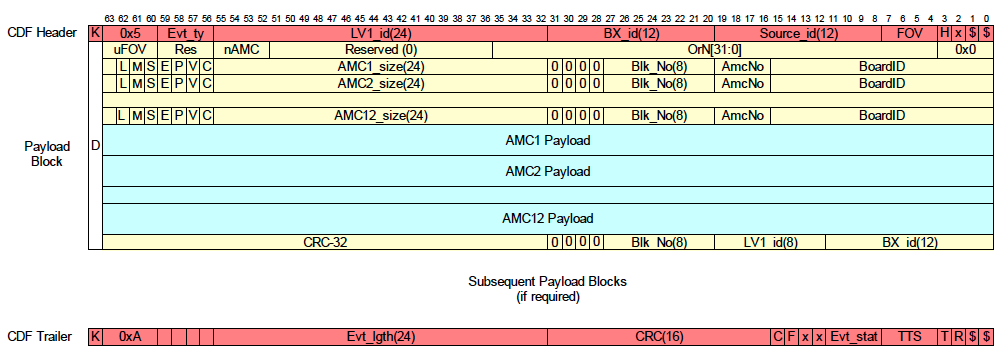
\includegraphics[width=7.5in]{images/amc13_output.png}
\caption{AMC13 to DAQ data format.}
\label{amc13-output}
\end{figure}

\section{FC7 Data Format}

The AMC13 imposes further specifications on the format of the data sent from the FC7.  In particular, it requires its own two headers and one trailer to surround the FC7 data.

The format of the FC7 data block differs slightly depending on whether the FC7 is for TTC encodement or fanout, as shown in Figures~\ref{efc7-to-amc13} and \ref{ffc7-to-amc13}, respectively.  A brief description of the main parameters is given in Table~\ref{tab:fc7-vars}.

\vspace*{3em}

\begin{figure}[h]
\hspace{-0.5in}
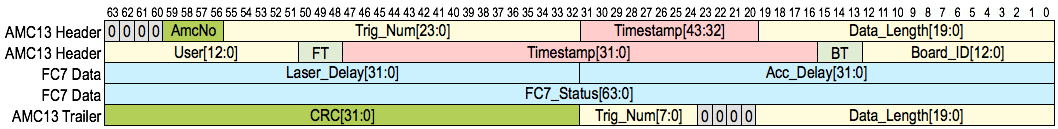
\includegraphics[width=7.5in]{images/encoder_fc7_data_format.png}
\caption{Encoder FC7 to AMC13 data format.}
\label{efc7-to-amc13}
\end{figure}

\begin{figure}[h]
\hspace{-0.5in}
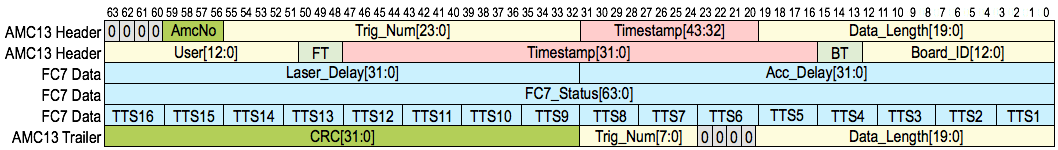
\includegraphics[width=7.5in]{images/fanout_fc7_data_format.png}
\caption{Fanout FC7 to AMC13 data format.}
\label{ffc7-to-amc13}
\end{figure}

{
\renewcommand{\arraystretch}{1.25}
\begin{table}[p]
\begin{center}
\begin{tabular}{| p{1.1in} | p{5in} |}
\hline
Parameter & Description \\ \hline \hline
\verb|AmcNo| & AMC slot number occupied by the FC7, indexed from 1 to 12.  Inserted by the AMC13. \\ \hline
\verb|Trig_Num| & TTC trigger number.  This is not the same as a ``muon fill number'' because laser and pedestal triggers will also be included in the overall count.  If needed, a separate fill counter for muon fills could incorporated and stored in the \verb|User| parameter. \\ \hline
\verb|Timestamp| & There is a 44-bit counter that is incremented in the FC7 on the rising edge of the 40-MHz TTC clock.  This field is the value of that counter when each TTC trigger is received off the \uTCA backplane.  Note that, with a 44-bit counter incrementing every 25~ns, it will not need to be reset for up to 5 days.  If needed, this counter can be setup to be reset for every run. \\ \hline
\verb|Data_Length| & Number of 64-bit words in the event, including the two AMC13 headers and one AMC13 trailer. \\ \hline
\verb|User| & 13 bits left available for the user. \\ \hline
\verb|FT| & 3-bit fill type, which will be \verb|001| for a muon fill, \verb|010| for a laser fill, and \verb|011| for a pedestal fill. \\ \hline
\verb|BT| & 3-bit board type, which will be \verb|001| for the Rider, \verb|010| for the CCC FC7, and \verb|011| for the tracker FC7. \\ \hline
\verb|Board_ID| & Unique serial number for the FC7 baseboard.  This number should be stored in an EEPROM, if available, and used to assign the MAC address. The MSB is reserved to distinguish between the TTC encodement (\verb|0|) and the TTC fanout (\verb|1|) FC7 boards. \\ \hline
\verb|Laser_Delay| & Delay set for the output trigger to the laser system, in units of the number of 40-MHz TTC clock cycles. \\ \hline
\verb|Acc_Delay| & Delay set between the received accelerator trigger and the output TTC trigger, in units of the number of 40-MHz TTC clock cycles. \\ \hline
\verb|FC7_Status| & 64 bits available for the important FC7 status signals.  This will include internal errors, such as from the SFP transceivers, and the trigger sequence index number. \\ \hline
\verb|TTS#| & Latest TTS state received from the given SFP receiver. \\ \hline
\verb|CRC| & Checksum inserted by the AMC13 for an offline data integrity check. \\ \hline
\end{tabular}
\end{center}
\caption{FC7 parameters that appear in its output data format.}
\label{tab:fc7-vars}
\end{table}
}
